\section{Crowdsourcing Task Interfaces}\label{sec:crowdsourcing_task_interfaces}
In this section some example interfaces are presented which were shown to crowd workers for each verification task. 

After selecting the concepts for ontology validation, the plugin automatically creates the relevant crowdsourcing jobs. Only Figure~Eight is currently supported as target crowdsourcing platform. Depending on the method of context enrichment~(see \hyperref[chap:context_enrichment_methods]{Chapter~\ref*{chap:context_enrichment_methods}}) different crowdsourcing interfaces were generated, as illustrated in \hyperref[fig:all_crowdsourcing_interfaces]{Figure~\ref*{fig:all_crowdsourcing_interfaces}}. 

\begin{figure}
    \centering
    \begin{subfigure}[b]{\textwidth}
        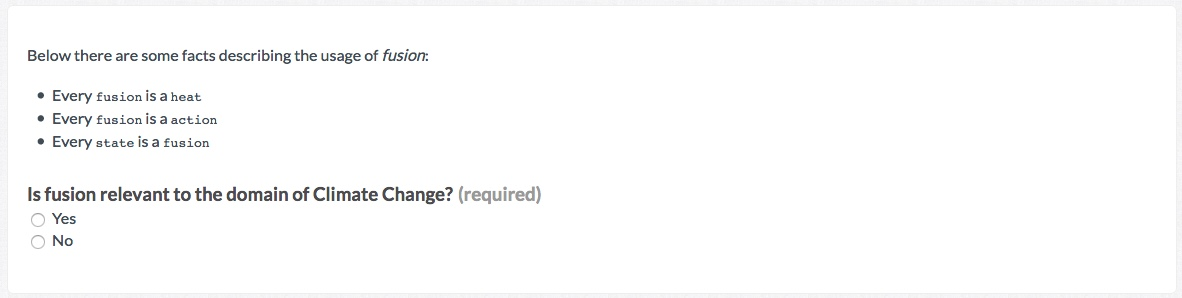
\includegraphics[width=\textwidth]{screenshots/questionaire_subclass_relation_context_enrichment}
        \caption{Neighbouring Nodes}
        \label{fig:crowdsourcing_interface_nn}
    \end{subfigure}
	~\\~\\
    \begin{subfigure}[b]{\textwidth}
        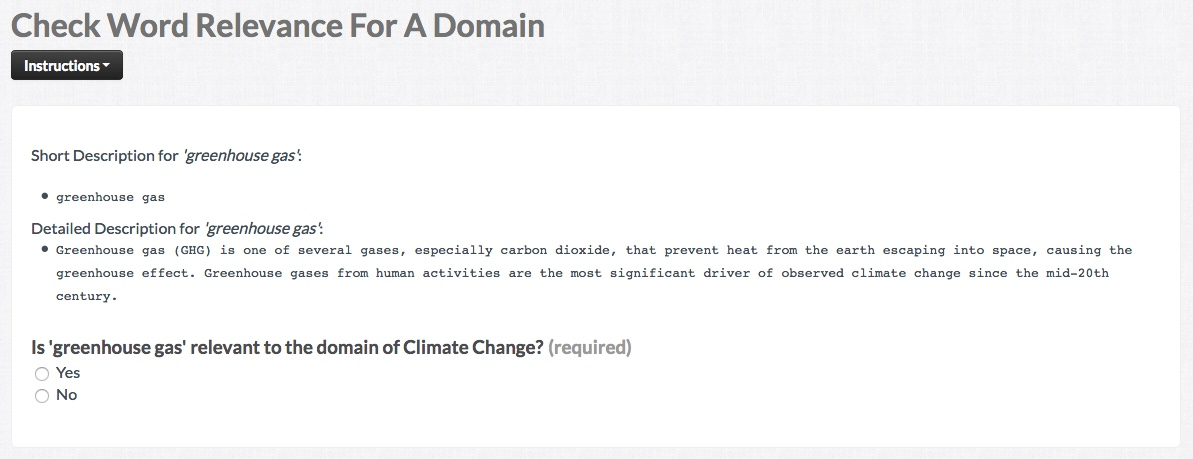
\includegraphics[width=\textwidth]{screenshots/questionaire_embedded_context_enrichment}
        \caption{Embedded Context}
        \label{fig:crowdsourcing_interface_ec}
    \end{subfigure}
	~\\~\\
    \begin{subfigure}[b]{\textwidth}
        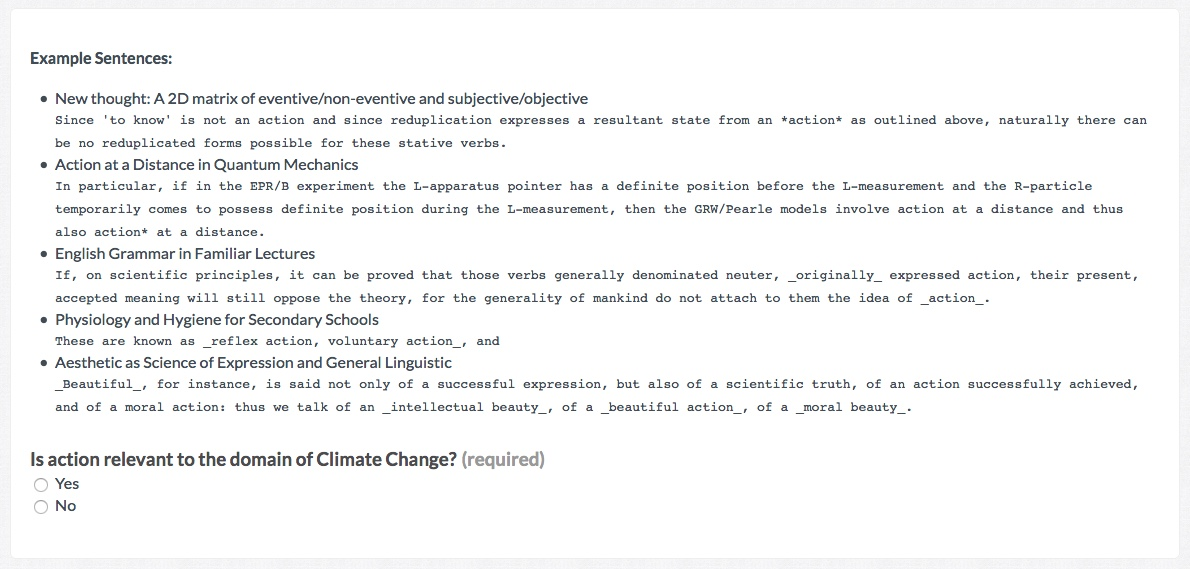
\includegraphics[width=\textwidth]{screenshots/questionaire_wordnik_context_enrichment}
        \caption{External Source}
        \label{fig:crowdsourcing_interface_es}
    \end{subfigure}
    \caption{Crowdsourcing task interfaces for performing ontology validation using different methods of context enrichment}\label{fig:all_crowdsourcing_interfaces}
\end{figure}

Each crowdsourcing interface consists of
\begin{enumerate}
		\item the instruction part
		\item the context part
		\item the question part
\end{enumerate}

The \emph{instructions} are relatively generic and therefore independent of the chosen context enrichment method. It contains a short description of the task goals and some examples of already answered verification questions. We paid attention to omit the details of ontology validation because first, it would confuse contributors and second, it is not relevant for answering the question. Also, we advised them to browse the Web or contact Wikipedia in case they do not know the answer or are unsure. It encourages contributors to give answers to their best knowledge and increases the quality of the responses at the same time. 

